
\graphicspath{ {figures/introduction/} }

%%%%%%%%%%%%%%%%%%%%%%%%%%%%%%%%%%%
\chapter{Introduction}
\label{ch:intro}

The natural world presents a stunning variety of multicellular organisms. We tend to distinguish them by their physiological traits. After all, we recognize penguins by their unusual stature, black and white fur, long beak, and impressive ability to wobble around on ice. These stereotyped features are a culmination of many complex cellular processes, collectively known as \emph{development}.

Development begins with a single cell, with subsequent growth and division events driving progression toward adulthood. Cells acquire increasingly specific roles and functions as growth proceeds, ultimately giving rise to stereotyped adult morphologies. This process, known as lineage restriction, demands that each cell decides to pursue the correct fate at the appropriate time and place \cite{Wilkins1993}.

Cell fate decisions are remarkably robust, collectively yielding consistent phenotypes amidst the vast array of conditions encountered in natural environments. They are so reliable that we often take them for granted. After all, it is hard to imagine a scenario in which we might mistake another human for a penguin. However, they can and do make mistakes with dire consequences for human health \cite{Immuno2010,Wang2009,Hornberg2006}. Researchers therefore continue to study these complex processes in the hope that they might one day be able to control their behavior; either to exploit them in novel biotechnologies, or rectify the diseases that arise when they fail. Research efforts are predominantly motivated by two fundamental questions. First, how do cells make decisions? Second, how do they make them reliably? 

This dissertation addresses subtle aspects of both questions by combining chemical engineering, computer vision, and statistics to extract meaningful insight from experimental data. The remaining sections of this chapter serve to prime the reader with the context needed to situate the presented findings within the broader literature. 

\section{Molecular origins of cell fate decisions}

Early experiments in the common fruit fly demonstrated that developmental processes are encoded in the genome \cite{Morgan1915a,Beadle1936}. Genetics were therefore believed to provide a predefined road map for a the journey from embryo to adulthood, inspiring researchers throughout the twentieth century to probe the roles of individual genes in coordinating adult phenotypes \cite{Lewis1978,Nusslein-Volhard1980,Halder1995}. Most of their efforts embraced a common philosophy; break something and see what happens. In \emph{Drosophila}, the genes themselves bare the legacy of this approach, as they are predominantly named after the phenotypes that emerge in their absence. Perturbing \textit{eyeless} or \textit{wingless} may now seem rudimentary, but these types of genetic perturbations were vital to the discovery of genetic components and architectures that dictate cell fate decisions in all organisms \cite{Halder1995,Perrimon1994,Bellen2010}. They revealed that some genes confer pleiotropic functions across several stages of development, while others are limited to a single context \cite{Parody1993a,Perrimon1994,IanSimpson2002a}. They also showed that some genes are only essential for proper development when others are absent, making them unnecessary under normal conditions \cite{Bhanot1999,Pappu2005,Li2005}. Moreover, \emph{Drosophila} continues to be a prominent model system for studying developmental processes today, owing to its conveniently short life cycle, wealth of prior knowledge, and deep library of available genetic machinery \cite{Beira2016,Enomoto2018,Germani2018}.

Among these tools, gene-specific reporters augment traditional genetic perturbations by providing localized readouts of transcript and protein abundance. Researchers can now break something and see what happens to specific components of the developmental program. Reporters have proven particularly useful for monitoring the activities of transcription factors; proteins that bind the promoter region of other genes in order to modulate their expression. Multiple transcription factors may interact with each other, allowing for the assembly of gene regulatory networks (GRN) that integrate upstream signaling cues to elicit specific changes in gene expression \cite{Levine2005,Stathopoulos2005}. 

GRNs thus arm cells with a chemical mechanism to orchestrate cell fate decisions in space and time. A prominent example occurs during the during the earliest stages of \textit{Drosophila} embryogenesis, where spatial morphogen gradients drive variegated expression of the Gap genes \cite{Hulskamp1990,Hulskamp1991}. The expressed proteins trigger subsequent developmental events in a concentration-dependent manner, inducing localized cascades of GRN activity that ultimately give rise to distinct morphological segments \cite{Johnston1992}. The embryonic landscape of Gap gene expression thereby defines a template for later stages of patterning. Developmental success is contingent upon GRNs tightly controlling the spatial precision of the template over time \cite{Perry2011}. Thus, segment polarity definition exemplifies a broader role of GRNs; they confer positional information to inform downstream cell fate decisions \cite{Struhl1993a}.

The resolution of positional information is thought to be refined over time. This assertion is in part based on experimental studies of retinal patterning in the \textit{Drosophila} eye, a setting with an enduring experimental legacy that continues to garner attention \cite{Bellen2010,Beira2016}. It remains popular in part because the temporal history of cell fate decisions is visibly encoded in the eye imaginal disc. During the third larval instar, a wave of differentiation steadily progresses across a disordered pool of multipotent cells (Fig. \ref{fig:intro:retinal_patterning}A) \cite{Ready1976a,Tomlinson1987a}. Differentiating cells propagate this morphogenetic furrow (MF) by relaying extracellular cues downstream. Decades of experiments have steadily revealed how cells interpret the signals and commit to particular fates (Fig. \ref{fig:intro:retinal_patterning}B) \cite{Voas2004}. Fate-specific reporters have shown that R8 photoreceptor neurons are recruited from pools of multipotent cells at the leading edge of the furrow \cite{Jarman1994}. The first cell to differentiate uses paracrine signaling to inhibit differentiation among its neighbors, resulting in a repeated pattern of regularly-spaced R8 cells that gives rise to the crystalline lattice structure of the adult eye \cite{Frankfort2002a}. The process dynamically transforms a disordered collection of cells into an ordered template for subsequent stages of patterning. In other words, it refines the spatial resolution of the developing eye field.

\begin{figure}[h!]
\centering
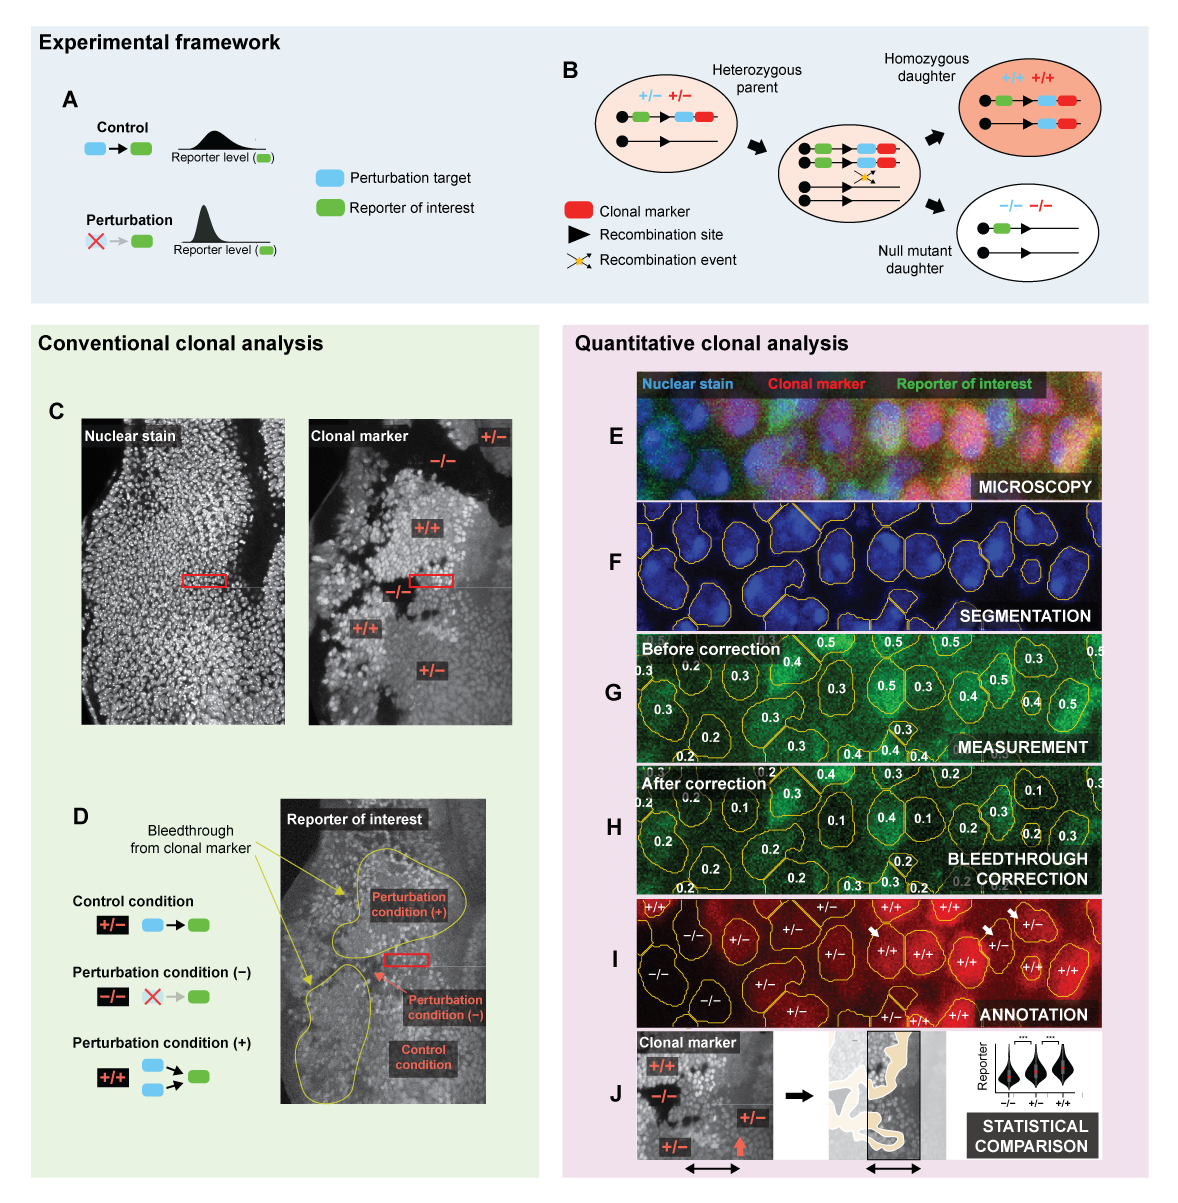
\includegraphics[width=\textwidth]{./figure_1}
\caption[Retinal patterning in \emph{Drosophila}.] {\textbf{Retinal patterning in \emph{Drosophila}.} (A) Differentiation is initiated in the developing eye by the MF, which moves across the eye epithelium from posterior to anterior (white arrow). On the furrow's posterior side, G1-arrested progenitor cells differentiate (light blue). Formation of regularly spaced R8 photoreceptors (red dots) precedes recruitment of additional R cell types (yellow dots). On the anterior side, progenitor cells are still proliferating (dark blue). Axis refers to time elapsed since fertilization. Adapted from Pel\'{a}ez et al. (2015). (B) Top, cartoon of an apical view of the sequential differentiation of eight R cell types from multipotent progenitor cells (grey) and their relative positions within a single ommatidium. Arrows denote signals transmitted from the R8 to nearby cells. Bottom, a cross-section view through an eye disc, showing the epithelial constriction that marks the MF (boxed region) and then the relative nuclear positions of progenitors (grey) and specified R cells (various colors). Both panels are adapted from Pel\'{a}ez et al. (2015).}
\label{fig:intro:retinal_patterning}
\end{figure}

Experiments suggest cell decisions to commit to an R8 fate are non-deterministic. Differentiation is driven by the expression of Atonal, a transcription factor initially induced in all cells along the leading edge of the furrow \cite{Jarman1994,Baker1997,Hsiung2002}. Stochastic differences in cells reception of signaling cues yields variation in Atonal levels and, consequently, cells propensities to adopt an R8 fate \cite{Baker1990,Gavish2016}. The eventual R8 cell therefore does not appear to be predetermined. Equivalent mechanisms have been shown to control many other cell fate decisions, including sensory bristle specification and the choice between epidermal and neural fates in the neuro-ectoderm of \textit{Drosophila} \cite{Ghysen1993,Simpson1997}.

These examples expose another important feature of GRNs: their output is non-deterministic. Dual-reporter experiments in \emph{E. coli} have elegantly shown that variation may be attributed to intrinsic thermal fluctuations at the molecular scale, as well as extrinsic variation in cell state \cite{Elowitz2002}. Both types of noise have since been shown to manifest in the population-wide penetrance of complex organismal phenotypes \cite{Raj2010,Paulsen2011,Burga2011,Colman-Lerner2005}. Some developmental systems appear to leverage noise, using GRNs to amplify and reinforce stochastic fluctuations in order to limit signal responses to a randomly chosen subset of cells \cite{Baker1990,Ghysen1993,Simpson1997}. Indeed, Pel'{a}ez et al. recently speculated that a similar mechanism may explain why subsequent R cell fate transitions coincide with rapid increases in transcription factor expression heterogeneity \cite{Pelaez2015a}.

These experiments and others like them form our contemporary systems-level view of development, in which complex networks of regulatory interactions guide cells toward the appropriate fates by refining their stochastic behavior over time. However, it is unknown precisely how cell fates are resolved from the dynamic activities of GRNs. It is also unclear how cells integrate stochastic inputs to execute reliable cell fate decisions. These ambiguities persist despite the wealth of experimental data generated throughout the past century. New approaches are therefore needed to unravel the complexities of GRNs and their execution of cell fate decisions.

\section{The power of quantitative analysis}

Experimental perturbations continue to supply some of the most potent tools in the arsenal available to researchers, but it has become clear that quantitative and systematic analysis frameworks are needed to tease apart the complex interactions that govern cell fate decisions \cite{Lazebnik2004,Oates2009}. Moreover, attempts to either rectify faulty decision mechanisms or engineer new ones, such as for cancer treatment or the generation of induced pluripotent stem cells, demand predictive models backed by quantitative data \cite{Hornberg2006}.

The focus has therefore gradually shifted from break something and \textit{see} what happens to break something and \textit{measure} what happens. The transition is supported by simultaneous advances in the resolution with which we can quantify GRN activity during development. Early approaches assayed the aggregate transcript or protein content of entire tissues. Strategies have since diverged in three separate directions, each of which sharpens the focus to single-cell resolution while prioritizing a different dimension of measurement. First, high-throughput transcriptomics strategies emphasize the breadth of genes surveyed. Second, flow cytometric approaches stress measurement precision. In both cases, cells identities may be crudely inferred from lineage-specific barcodes or biomarkers \cite{Herring2018}, but the precise spatial identify of each cell is discarded. In contrast, methods based on quantitative microscopy prioritize spatial resolution because cells are measured in their native context. These techniques generally entail imaging gene-specific fluorescent reporters before using software to detect individual cells and quantify their fluorescence levels. They are particularly well-suited to probing the intricacies of GRNs subject to signaling from adjacent cells, and have consequently become a preferred option for studying tissue-scale patterning. In terms of microscopy, the state of the art has steadily progressed from static ex vivo imaging of fixed tissues to in situ recording of single-cell expression dynamics \cite{Keller2013}. Computational methods to support quantitative image analysis have enjoyed similar progress \cite{Sbalzarini2016}. Combined, these advances allow researchers to collect the data needed to conduct rigorous analyses and make testable predictions \cite{qbio2018}. That is, they promote quantification.

Quantification has completely redefined the precision of GRN analysis. The enhanced resolution has inspired exciting new research into the specific mechanisms of information transmission and processing that underlie cell fate decisions in a broad variety of model systems \cite{Pelaez2015a,Frick2017,Wolff2018,Petkova2019}. These pursuits have also emboldened researchers to pause and reconsider canonical wisdom. Petkova et al. recently combined quantitative dynamic measurements and information theory to show that gap gene expression provides sufficient spatial context to uniquely define the positions of all cells \cite{Petkova2019}. The authors argued that downstream GRNs likely decode these signals with near-optimal efficiency, implying that many cell fates could, at least in principle, be determined during the earliest stages of \emph{Drosophila} embryogenesis. The findings imply that the resolution of positional information does not necessarily need to be refined as development proceeds. Similarly, cell fates need not be spatially resolved over time, prompting closer scrutiny of the extent to which cell fate decisions during later stages of development are truly non-deterministic. In causing the field to revisit these tenets of established dogma, the study exemplifies the power of quantification to produce novel insight.

Despite its revelatory potential, biologists have not universally embraced quantification, instead continuing to rely on visual analysis of imaging data. Resistance may partially come down to the scarcity of computational proficiency in experimental labs. Collaborations help alleviate this bottleneck, but they are often plagued by long turnaround times as researchers attempt to juggle many unrelated commitments. User-friendly analysis software would benefit experimentalists caught in this predicament by eliminating the need for computational proficiency altogether. Automated analysis frameworks have already played a similar role in many other subdisciplines of biology \cite{Aghaeepour2013,Chen2015,Pyne2009,Bernstein2008,Hellemans2007,Langmead2012,Trapnell2009,Costes2004,Kelley2015,Carpenter2006,Paintdakhi2016,Schindelin2012,Sommer2011}. Indeed, without the support of automated alignment software, next-generation sequencing would be inaccessible to all but a few labs with extensive programming and statistical modeling experience. Similar platforms are available to support quantification of microscopy data \cite{Schindelin2015,Sbalzarini2016}, but comparatively few are tailored to address the intricacies of specific model systems and experimental pipelines \cite{Jug2014}. Further development of context-specific quantification platforms is therefore needed in order to lower the barrier to adoption of data-driven analysis.

\section{Mathematical modeling of cell fate decisions}

Mathematical models have reinvigorated the study of cell fate decisions in a broad variety of contexts. Most modeling efforts fall into one of two categories; those that use a data-driven approach to recapitulate molecular mechanism, and those that provide a sparse representation of systems-level behavior. 

The first class of models strive to parameterize specific biomolecular interactions by fitting a model directly to data. They typically describe the time-evolution of transcripts and proteins using systems of coupled ordinary differential equations (ODEs) reminiscent of those familiar to chemical engineers and ecologists. Despite the illusion of mechanistic detail, these models still deploy a healthy dose of abstraction. None of the commonly used rate represent true elementary reactions, instead opting for empirical representations such as linear degradation and cooperative binding kinetics. Nevertheless, many novel GRN behaviors and functions have been elegantly proposed and tested in this manner \cite{Barkai1997b,Yu2008a,Paulsen2011}. 

The second class of models forego molecular detail in favor of a coarse-grained representation of a particular phenomenon. These approaches provide a powerful means to identify, characterize, and predict behaviors that span a broad variety of model systems and developmental contexts. Among the common modeling frameworks, control theory has proven particularly fertile for generating and testing hypotheses related to GRN dynamics. Bacterial chemotaxis offers a compelling example in which molecular models were supplanted by a simple integral control framework \cite{Barkai1997b,Alon1999,Yi2000,Muzzey2009}. Analogous strategies have drawn inspiration from several disciplines to discover numerous novel functions of GRNs \cite{Ma2009,Colman-Lerner2005,Rahimi2016,Benzinger2018,Adler2018,Yordanov2018}.

Coarse-grained models are particularly well suites to studying how cell fates are resolved from spatiotemporal signaling cues. These problems would otherwise be intractable due to the many complex transport processes that shuttle signaling molecules between neighboring cells. Lubensky et al. developed a relatively simple reaction-diffusion approach to model pattern formation in the larval eye. They showed that inductive signaling cues could drive cell-autonomous positive feedback to account for the emergence of a hexagonal lattice of R8 cells, as well as an otherwise inexplicable striped pattern observed in some mutants \cite{Lubensky2011}. Gavish et al. used an even simpler model to show that an additional inhibitory signal is required to stabilize retinal patterning against minor fluctuations in cells spatial arrangement. The authors then used an experimental technique known as quantitative mosaic analysis to identify the unknown diffusible inhibitor \cite{Gavish2016}.

Mathematical models have also shone light on the regulatory interactions that implement cell fate decisions within individual cells. One study explored how cells generate all-or-none responses to morphogen gradients in the \emph{Drosophila} ventral ectoderm \cite{Melen2005}. An ultrasensitive response mechanism was proposed to dictate the expression of Yan, a transcriptional repressor known to impede cell fate transitions \cite{Lai1992a,Rogge1995,Rebay1995}. A later study proposed that Yan plays a different role in the larval eye, instead forming a bi-stable switch through reciprocal antagonism with a transcriptional activator named Pointed (Pnt) \cite{Graham2010}. The authors used a psuedo-molecular model to demonstrate that the decision to adopt an R cell fate could be triggered by an irreversible transition between two stable states; one characterized by high Yan and low Pnt expression, and the other by low Yan and high Pnt expression. Both transcription factors are known to be subject to several seemingly redundant sources of negative feedback. The model rationalized the purpose of these inhibitors by postulating that they enforce bi-stability of the two distinct states. Transitions between the states are triggered by an increase in Pnt levels. Shwartz et al. extended the model to include autoregulatory interactions that help flip the switch by converting transient inductive signals into sustained Pnt expression \cite{Shwartz2013}.

Soon thereafter, the advent of a Pnt-specific fluorescenct reporter curiously revealed that Yan and Pnt are co-expressed in several developmental contexts \cite{BoisclairLachance2014}. Pel\'{a}ez et al. then published quantitative measurements indicating Yan exhibits  mono-stable expression dynamics in the larval eye \cite{Pelaez2015a}. These two studies fundamentally contradict the existing model, prompting renewed interest in both Yan and Pnt. Namely, how do they cooperate to mediate cell fate decisions? How do they do so reliably? And why are they subject to so much negative feedback?

\section{Roles for negative feedback in GRNs}
 
Theory supports many potential uses for negative feedback in developmental GRNs \cite{Freeman2000}. Perhaps the most obvious application is the maintenance of cell states --- that is, rejecting exogenous disturbances and driving cells toward a desired set point \cite{Alon2007,Behar2007,Yi2000}. Negative feedback has also been shown to improve information transmission by linearizing input-output relationships and expanding dynamic range in several developmental signaling cascades \cite{Bhalla2002,Cheong2011,Paulsen2011,Yi2003,Yu2008a}. Yi et al. used a FRET-based reporter of the G\textalpha-subunit to demonstrate dose-response alignment of G-protein signaling activity at the highest level of the yeast mating response pathway \cite{Yi2003}. Yu et al. later quantified pFus3 activity to show that negative feedback further increases signal fidelity throughout much of the downstream pathway \cite{Yu2008a}. These functions mimic critical roles for negative feedback in human-engineered systems \cite{Khammash2016}.

Negative feedback is also vital to the reliable execution of cell fate decisions. Rahimi et al. showed that Wnt-mediated negative feedback enhances the precision of morphogen gradients in the ventral domain of the \textit{Drosophila} embryo \cite{Rahimi2016}. Paulsen et al. showed that the fidelity of BMP4 signaling in the \textit{Xenopus} embryo is improved by concomitant expression of a repressor that suppresses transduction of extrinsic noise. Eliminating the repressor leads to increased variation of pathway outputs, as well as the cell fate decisions they control \cite{Paulsen2011}. These studies provide direct experimental evidence that negative feedback can suppress phenotypic variation. 

Experiments in \emph{Drosophila} indicate that short non-coding transcripts, called microRNAs, confer a similar function by buffering developmental processes against both environmental and genetic variability \cite{Cassidy2016a,Cassidy2013,Li2009b,Ebert2012}. Li et al. studied the effect of perturbing miR-7 activity during sensory organ development, and found that the microRNA stabilizes both gene expression and fate commitment decisions against fluctuating environmental conditions \cite{Li2009b}. Cassidy et al. used directional selection to quantify the heritability of bristle formation defects in miR-9a mutants, revealing that microRNAs can also suppress the influence of intrinsic genetic variation \cite{Cassidy2013}. The same group later showed that miR-9 suppresses the penetrance of genetic variants deleterious to viability at elevated temperatures \cite{Cassidy2016a}. Negative feedback mediated by microRNAs has therefore been shown to directly affect the evolutionary fitness of adult organisms by promoting robustness against varying environmental conditions. Precisely how this effect is achieved remains unknown.

\section{Evolutionary drivers of robust cell fate decisions}

Studies of developmental robustness are often traced back to C.H. Waddington’s claim that “there is scarcely a mutant that is comparable in constancy with the wild type” \cite{Waddington1942}. His comment reflects the consistency of adult phenotypes amidst modest levels of genetic and environmental variation, which gives way to variation when severe perturbations are introduced \cite{Bateman1959a,Rendel1959,Rendel1966a,Scharloo1991}. Robustness has since been attributed to individual genes and their products \cite{Dun1958,Gibson1996,Rutherford1998}, as well as the systems-level architectures that they comprise \cite{Rutherford1998,Paulsen2011,Li2009b,Eldar2002,Denby2012,Cassidy2013,Cassidy2016a}. A handful of conserved regulatory motifs, and the strategies they implement, are now understood to pervade most developmental processes \cite{Freeman2000,Hartman2001,Alon2007,Marciano2014}. Robustness has thus come to be accepted as a fundamental organizational principle underlying the evolution of all biological systems \cite{Kitano2004,Stelling2004}. That is, selection for genotypes that confer robustness is widely assumed to shape the evolution of gene regulatory network topologies. 

The specific evolutionary drivers for increased robustness of GRNs remain unclear \cite{Siegal2014}. Citing phenomenological examples, Waddington attributed robustness to evolutionary selection for optimal traits. More recently, Siegal et al. argued that developmental robustness can arise without stabilizing selection for any particular phenotype \cite{Siegal2002}. They used a gene interaction network model to demonstrate that robustness is an emergent property of complex networks subject only to selection on the basis of their own functional stability. The same authors used in silico evolution to show that most genes in developmental networks buffer phenotypic variation, indicating that robustness may be an emergent byproduct of GRN architecture \cite{Bergman2003}. Computational studies have also questioned the notion that global GRN properties are a consequence of adaptive evolution, instead suggesting that local properties of genetic circuits could drive the emergence of macroscopic features, such as those that ensure robust development \cite{Lynch2007,Wagner2003}.

When a gene or its products are absent or fail to perform their functions, the simplest contingency is to have others ready to compensate. It consequently seems intuitive that cells could incorporate functional redundancy to guarantee reliable cell fate decisions \cite{Hartman2001,McAdams1999}. One computational study showed that genetic redundancy is particularly evolutionarily stable in developmental systems. By simulating functionally overlapping pairs of genes, the authors demonstrated that increasing the probability with which each gene independently fails to carry out its function places increasing selection pressure upon the pair as a whole \cite{Nowak1997}. They reasoned that the resultant increase in evolutionary stability explains the prevalence of redundancy in developmental systems, where failure rates are high and erroneous cell fate decisions yield deleterious phenotypes. Their suggestion is consistent with extensive documentation of functional redundancy in developmental systems \cite{Kitano2004}. 

Redundancy could arise through gene duplication or convergent evolution. A. Wagner argued against the former. He analyzed gene sequence and expression data in yeast to show that the phenotypic severity of loss-of-function mutations does not correlate with the availability of functionally equivalent genes. He concluded that functional redundancy is not the primary source of robustness against genetic variation, instead favoring epistatic interactions between otherwise unrelated gene products \cite{Wagner2000}. Combined, these studies suggest the prevalence of functional redundancy in GRNs may be driven by as-of-yet unknown forces.
